\Chapter{Data Preparation}\label{chapter:data-preparation}

In this chapter, I will discuss the datasets used in training the method presented in this thesis and the data augmentation techniques applied to them.
The quality and nature of the data are paramount for training robust deep learning models, particularly for complex tasks such as novel view synthesis. This chapter details the meticulous process of curating and preparing the datasets used for training and validating the proposed method, with a primary focus on the extensive ObjaverseXL dataset used for training and the complementary Google Scanned Objects dataset used for validation.

\section{Dataset Overview}\label{sec:dataset-overview}

Two primary datasets form the backbone of this work: ObjaverseXL, a large-scale repository of 3D models utilized for training the generative model, and Google Scanned Objects (GSO), a collection of high-fidelity 3D scans employed in my work for validation purposes.

\subsection{ObjaverseXL: A Large-Scale 3D Model Repository}\label{ssec:objaversexl-overview}
ObjaverseXL \cite{objaversexl} is a vast, publicly accessible dataset comprising approximately 10 million 3D models. In order to use these models, one has to download them from their respective sources, which are often not straightforward. The models are stored in diverse online sources, including platforms like GitHub, Thingiverse, and Sketchfab, as shown in \ref{fig:objaversexl-overview}, resulting in a rich and varied collection that reflects a wide array of object categories, complexities, and artistic styles. Given its scale and diversity, ObjaverseXL serves as the primary source for the training data in this thesis.

\begin{figure}[h]
  \centering
  \includegraphics[width=0.5\textwidth]{images/data/sankey-diagram-objaverse-sources.png}
  \caption{Illustrative overview of ObjaverseXL model sources and diversity.}
  \label{fig:objaversexl-overview}
\end{figure}

\subsection{Google Scanned Objects (GSO): High-Quality 3D Scans}\label{ssec:gso-overview}
The Google Scanned Objects (GSO) dataset \cite{gso} consists of high-fidelity 3D scans of real-world objects. In this work, the GSO dataset is utilized for the final validation of the trained multi-view image generation model. Its distinct origin and capture methodology compared to ObjaverseXL provide a benchmark for evaluating the generalization capabilities and output quality of the proposed method on unseen, high-quality data.

\section{Processing Pipeline for ObjaverseXL Training Data}\label{sec:objaversexl-pipeline}
The transformation of raw 3D models from ObjaverseXL into a usable training dataset involved a comprehensive processing pipeline. This pipeline encompassed several critical stages: model acquisition, normalization, view rendering with specific lighting considerations, quality control filtering, and finally, textual annotation. Each step was carefully designed to address potential issues and ensure the final dataset's suitability for training an effective multi-view diffusion model.

\subsection{3D Model Acquisition and Initial Handling}\label{ssec:model-acquisition}
The first step involved acquiring the 3D models from their respective sources as listed in the ObjaverseXL dataset. This task required scripting the download process due to the varied hosting platforms. The pipeline was designed to robustly handle common 3D model formats that typically support textures, including Object files ($.obj$), GLTF/GLB files ($.glb$, $.gltf$), Filmbox files ($.fbx$), and Collada files ($.dae$).

A critical part of initial handling was standardizing the coordinate system. 3D models from diverse origins often have different conventions for which axis represents "up". To ensure consistency, all imported mesh objects underwent a corrective rotation of -90 degrees around the X-axis. This transformation was immediately applied to the objects, establishing a common "Z-up" orientation for all models before subsequent processing steps. A preliminary inspection of model metadata was also performed upon successful download, which sometimes provided hints for orientation if the automated correction was insufficient, though the Z-up convention was paramount.

\subsection{3D Model Normalization and Scene Setup}\label{ssec:model-normalization}
To ensure consistency across all rendered images, a standardized scene setup was imperative. Each downloaded 3D model underwent a normalization process:
\begin{enumerate}
  \item \textbf{Global Bounding Box Calculation}: The process began by calculating a single bounding box encompassing all mesh components of the loaded 3D model.
  \item \textbf{Scaling to Unit Cube}: Based on the maximum dimension of this global bounding box, a uniform $scale_factor$ was determined. The model was then scaled by this factor to ensure it fit precisely within a 1x1x1 unit cube.
  \item \textbf{Centering at Origin}: After scaling, the model was translated so that the center of its global bounding box was positioned at the world origin (0,0,0).
\end{enumerate}
This normalization was critical for several reasons. Firstly, it ensured that objects, regardless of their original size, would fit within the camera's viewpoint. Secondly, it provided a consistent reference point for defining camera positions and distances, simplifying the multi-view rendering setup.

\subsection{Multi-View Image Rendering}\label{ssec:multi-view-rendering}
The core of the data generation process was rendering 2D images of each 3D model from multiple viewpoints.

\subsubsection{Rendering Environment}\label{sssec:rendering-environment}
All rendering tasks were performed using Blender \cite{blender}, a powerful open-source 3D creation suite. To automate and scale the process, Blender was operated in windowless (headless) mode. The BLENDER\_EEVEE rendering engine was chosen for its balance of speed and quality, making it suitable for generating a large volume of images. Render output was configured to $1024x1024$ pixels in $PNG$ format with $RGBA$ color mode, enabling transparency. The background was explicitly set to transparent.

Specific EEVEE settings were configured to balance quality and performance while ensuring clear depiction of the objects:
\begin{itemize}
  \item \textbf{Temporal Anti-Aliasing (TAA)}: Render samples set to 32 for smoother edges.
  \item \textbf{Ambient Occlusion (GTAO)}: Enabled to provide contact shadows and enhance perceived depth.
  \item \textbf{Bloom}: Disabled to prevent overly bright, glowing effects that could obscure object details.
\end{itemize}

\subsubsection{Camera Viewpoint Configuration}\label{sssec:camera-config}
Camera setup was designed for consistency and to provide a comprehensive view of the objects.
Key camera parameters included:
\begin{itemize}
  \item \textbf{Focal Length}: 35mm.
  \item \textbf{Sensor Width}: 32mm.
  \item \textbf{Camera Distance}: Cameras were positioned at a fixed distance of 1.8 Blender units from the world origin. Given the 1x1x1 object normalization, this distance ensured the object was well-framed.
  \item \textbf{Targeting}: A $TRACK_TO$ constraint was applied to the camera, compelling it to always point towards the world origin (0,0,0), keeping the object centered.
\end{itemize}

To train a model capable of understanding objects from various perspectives and generalizing to different numbers of input views, images were rendered from a randomly selected set of predefined camera angles for each model. Three configurations were used for $6$, $8$ and $12$ views, with specific azimuth (horizontal rotation) and elevation alternating between small positive and negative values to cover the object from all sides. The camera is focused on the origin. The placement is shown in \ref{fig:camera-setups} and \ref{fig:camera-setups-up}.

\begin{figure}[h]
  \centering
  \includegraphics[width=0.6\textwidth]{images/data/rendering-ortho.png}
  \caption{Example camera configurations for 8 views around an object.}
  \label{fig:camera-setups}
\end{figure}

\begin{figure}[h]
  \centering
  \includegraphics[width=0.5\textwidth, angle=180]{images/data/rendering-up.png}
  \caption{Camera configurations for 8 views around an object, visible from the top.}
  \label{fig:camera-setups-up}
\end{figure}

The choice of 6, 8, or 12 views for any given model was made randomly, with the dataset designed to have an approximately equal distribution of samples across these three groups. This strategy aimed to enhance the model's robustness to varying input view counts during inference. Azimuth angles were defined to be counter-clockwise around the object to ensure compatibility with methods of 3D reconstruction like InstantMesh \cite{instantmesh}.

\subsubsection{Lighting Strategy for Consistent Illumination}\label{sssec:lighting-strategy}
Lighting plays a critical role in the visual appearance of rendered objects. The example rendering scripts provided by the ObjaverseXL authors \cite{objaverse} employed a randomized lighting setup. While intended to introduce variability, this approach often resulted in images with harsh lighting, strong shadows, or scenes where the object was underexposed or even completely obscured because the light source was positioned unfavorably (e.g., behind the object relative to the camera). Such inconsistencies could negatively impact model training, potentially teaching the model to generate overly dark or inconsistently lit views.

To mitigate this, a revised, deterministic multi-point lighting strategy using four $SUN$ type lights was adopted. The primary goal was to achieve soft, even illumination across the object's surface, ensuring that its features were clearly visible from all rendered viewpoints.

The resulting images featured more consistently well-lit objects, reducing the likelihood of the diffusion model learning to arbitrarily darken parts of an object from perspectives different from the main light source direction in the input. This consistency is vital for learning accurate geometry and appearance.

\subsection{Post-Rendering Quality Control and Filtering}\label{ssec:quality-control}
Despite the controlled rendering setup, not all rendering attempts yielded high-quality images. Some 3D models were inherently problematic (e.g., incompatible formats, missing textures, non-manifold geometry), while others, due to their material properties or fine details, resulted in renders that provided little useful visual information (e.g., images consisting mainly of reflections, transparency artifacts, or indiscernible silhouettes). It was observed that approximately one-third of the initially rendered samples suffered from such quality issues.

To ensure the training data was of sufficient quality, a rigorous filtering process was implemented. This was based on a contrast score, calculated as the standard deviation of pixel intensities in the grayscale version of each rendered image. A minimum contrast threshold was established. If any of the rendered views for a particular 3D model fell below this threshold, the entire sample (the 3D model and all its associated renders) was discarded from the dataset. This strict approach ensured that only models with consistently clear and informative views were retained. After this filtering stage, approximately $20,000$ high-quality 3D model samples, each with its set of 6, 8, or 12 views, remained.

\subsection{Textual Prompt Generation via Multimodal LLM}\label{ssec:text-generation}
To fine-tune a text-to-image diffusion model, rich textual descriptions (prompts) corresponding to the visual content are essential. Since the ObjaverseXL models do not inherently come with such descriptive prompts, they needed to be generated. For this task, a state-of-the-art multimodal Large Language Model (LLM), Qwen2.5VL \cite{qwen25vl}, was employed. Qwen2.5VL is recognized for its strong performance in image description and visual question answering tasks.

The prompt generation process was as follows:
\begin{enumerate}
  \item For each 3D model, three views were randomly selected from its set of successfully rendered and filtered images.
  \item These three views were provided as parallel input to the Qwen2.5VL model.
  \item The LLM was tasked with analyzing these views and generating a single, comprehensive, and descriptive text prompt that accurately captured the essence of the 3D object depicted.
\end{enumerate}
This approach aimed to distill visual information from multiple perspectives into a rich textual description, providing effective conditioning for the diffusion model during training. The use of multiple views was intended to help the LLM form a more holistic understanding of the object compared to relying on a single view.

\section{Processing of Google Scanned Objects (GSO) Validation Data}\label{sec:gso-processing}
The Google Scanned Objects (GSO) dataset was processed with a similar pipeline to ensure consistency in evaluation. The primary steps involved:
\begin{enumerate}
  \item Downloading the GSO 3D models.
  \item Passing them through the same normalization, multi-view rendering (using the same camera configurations and lighting strategy), quality control filtering pipeline and textual prompt generation described in Section \ref{sec:objaversexl-pipeline}.
\end{enumerate}

\section{Training Dataset Characteristics}\label{sec:final-dataset-chars}
Following the comprehensive processing pipeline, the final datasets were prepared for model training and validation.
The ObjaverseXL training dataset consists of approximately 20,000 unique 3D models, each associated with a set of high-quality rendered views (6, 8, or 12 per model) and a descriptive textual prompt generated by Qwen2.5VL. This curated dataset provides a rich and diverse source of multi-view image-text pairs for training the diffusion model.

The GSO validation dataset comprises a set of consistently rendered views from the high-fidelity GSO models (approximately 1000 models), ready to be used for evaluating the performance of the trained model, particularly its ability to generalize to unseen objects and maintain multi-view consistency.
With these meticulously prepared datasets, the subsequent stages of model training and experimentation, as detailed in the following chapters, could proceed on a solid foundation.

\subsection{Dataset Statistics}\label{ssec:dataset-statistics}
This subsection presents a visual overview of key statistics derived from the processed ObjaverseXL dataset. These visualizations offer insights into the distribution of various data attributes, which are helpful in understanding the characteristics of the data used for training.

First, the distribution of the number of rendered views per 3D model is presented. As described in Section \ref{sssec:camera-config}, models were rendered with 6, 8, or 12 views, with an approximately equal distribution. The exact frequencies (after filtering) are shown in Table \ref{tab:render-count-distribution}.

\begin{table}[h]
  \centering
  \caption{Distribution of Render Counts per Model.}
  \label{tab:render-count-distribution}
  \pgfplotstabletypeset[
    col sep=comma,
    string type,
    columns/render_count/.style={column name=Render Count, column type=c},
    columns/frequency/.style={column name=Frequency, column type=c},
    every head row/.style={before row=\toprule, after row=\midrule},
    every last row/.style={after row=\bottomrule},
  ]{images/data/objaverse_visualizations/distribution_render_count_bar_data.csv}
\end{table}

Figure \ref{fig:dist-file-size} illustrates the distribution of file sizes (in Megabytes) of the original 3D models in the dataset.

\begin{figure}[h]
  \centering
  \includegraphics[width=0.9\textwidth]{images/data/objaverse_visualizations/distribution_file_size_bytes.png}
  \caption{Distribution of sample sizes in the ObjaverseXL dataset. Statistics: $\mu = 37.25$ MB and $\sigma = 117.93$ MB.}
  \label{fig:dist-file-size}
\end{figure}

The distribution of average image contrast across the rendered views is shown in Figure \ref{fig:dist-avg-contrast}. This metric was crucial for the quality control filtering process, as detailed in Section \ref{ssec:quality-control}.

\begin{figure}[h]
  \centering
  \includegraphics[width=0.9\textwidth]{images/data/objaverse_visualizations/distribution_average_contrast.png}
  \caption{Distribution of average contrast scores for rendered images. Statistics: $\mu = 36.97$ and $\sigma = 53.15$.}
  \label{fig:dist-avg-contrast}
\end{figure}

Figure \ref{fig:dist-prompt-length} displays the distribution of the lengths of textual prompts generated by the Qwen2.5VL model. These prompts are vital for conditioning the text-to-image diffusion model.

\begin{figure}[h]
  \centering
  \includegraphics[width=0.9\textwidth]{images/data/objaverse_visualizations/distribution_prompt_length.png}
  \caption{Distribution of generated prompt lengths. Statistics: $\mu = 476.06$ and $\sigma = 170.18$.}
  \label{fig:dist-prompt-length}
\end{figure}

A word cloud visualization of the most frequent terms appearing in the generated prompts is presented in Figure \ref{fig:wordcloud-prompts}. This offers a qualitative glimpse into the common themes and object characteristics described in the dataset.

\begin{figure}[h]
  \centering
  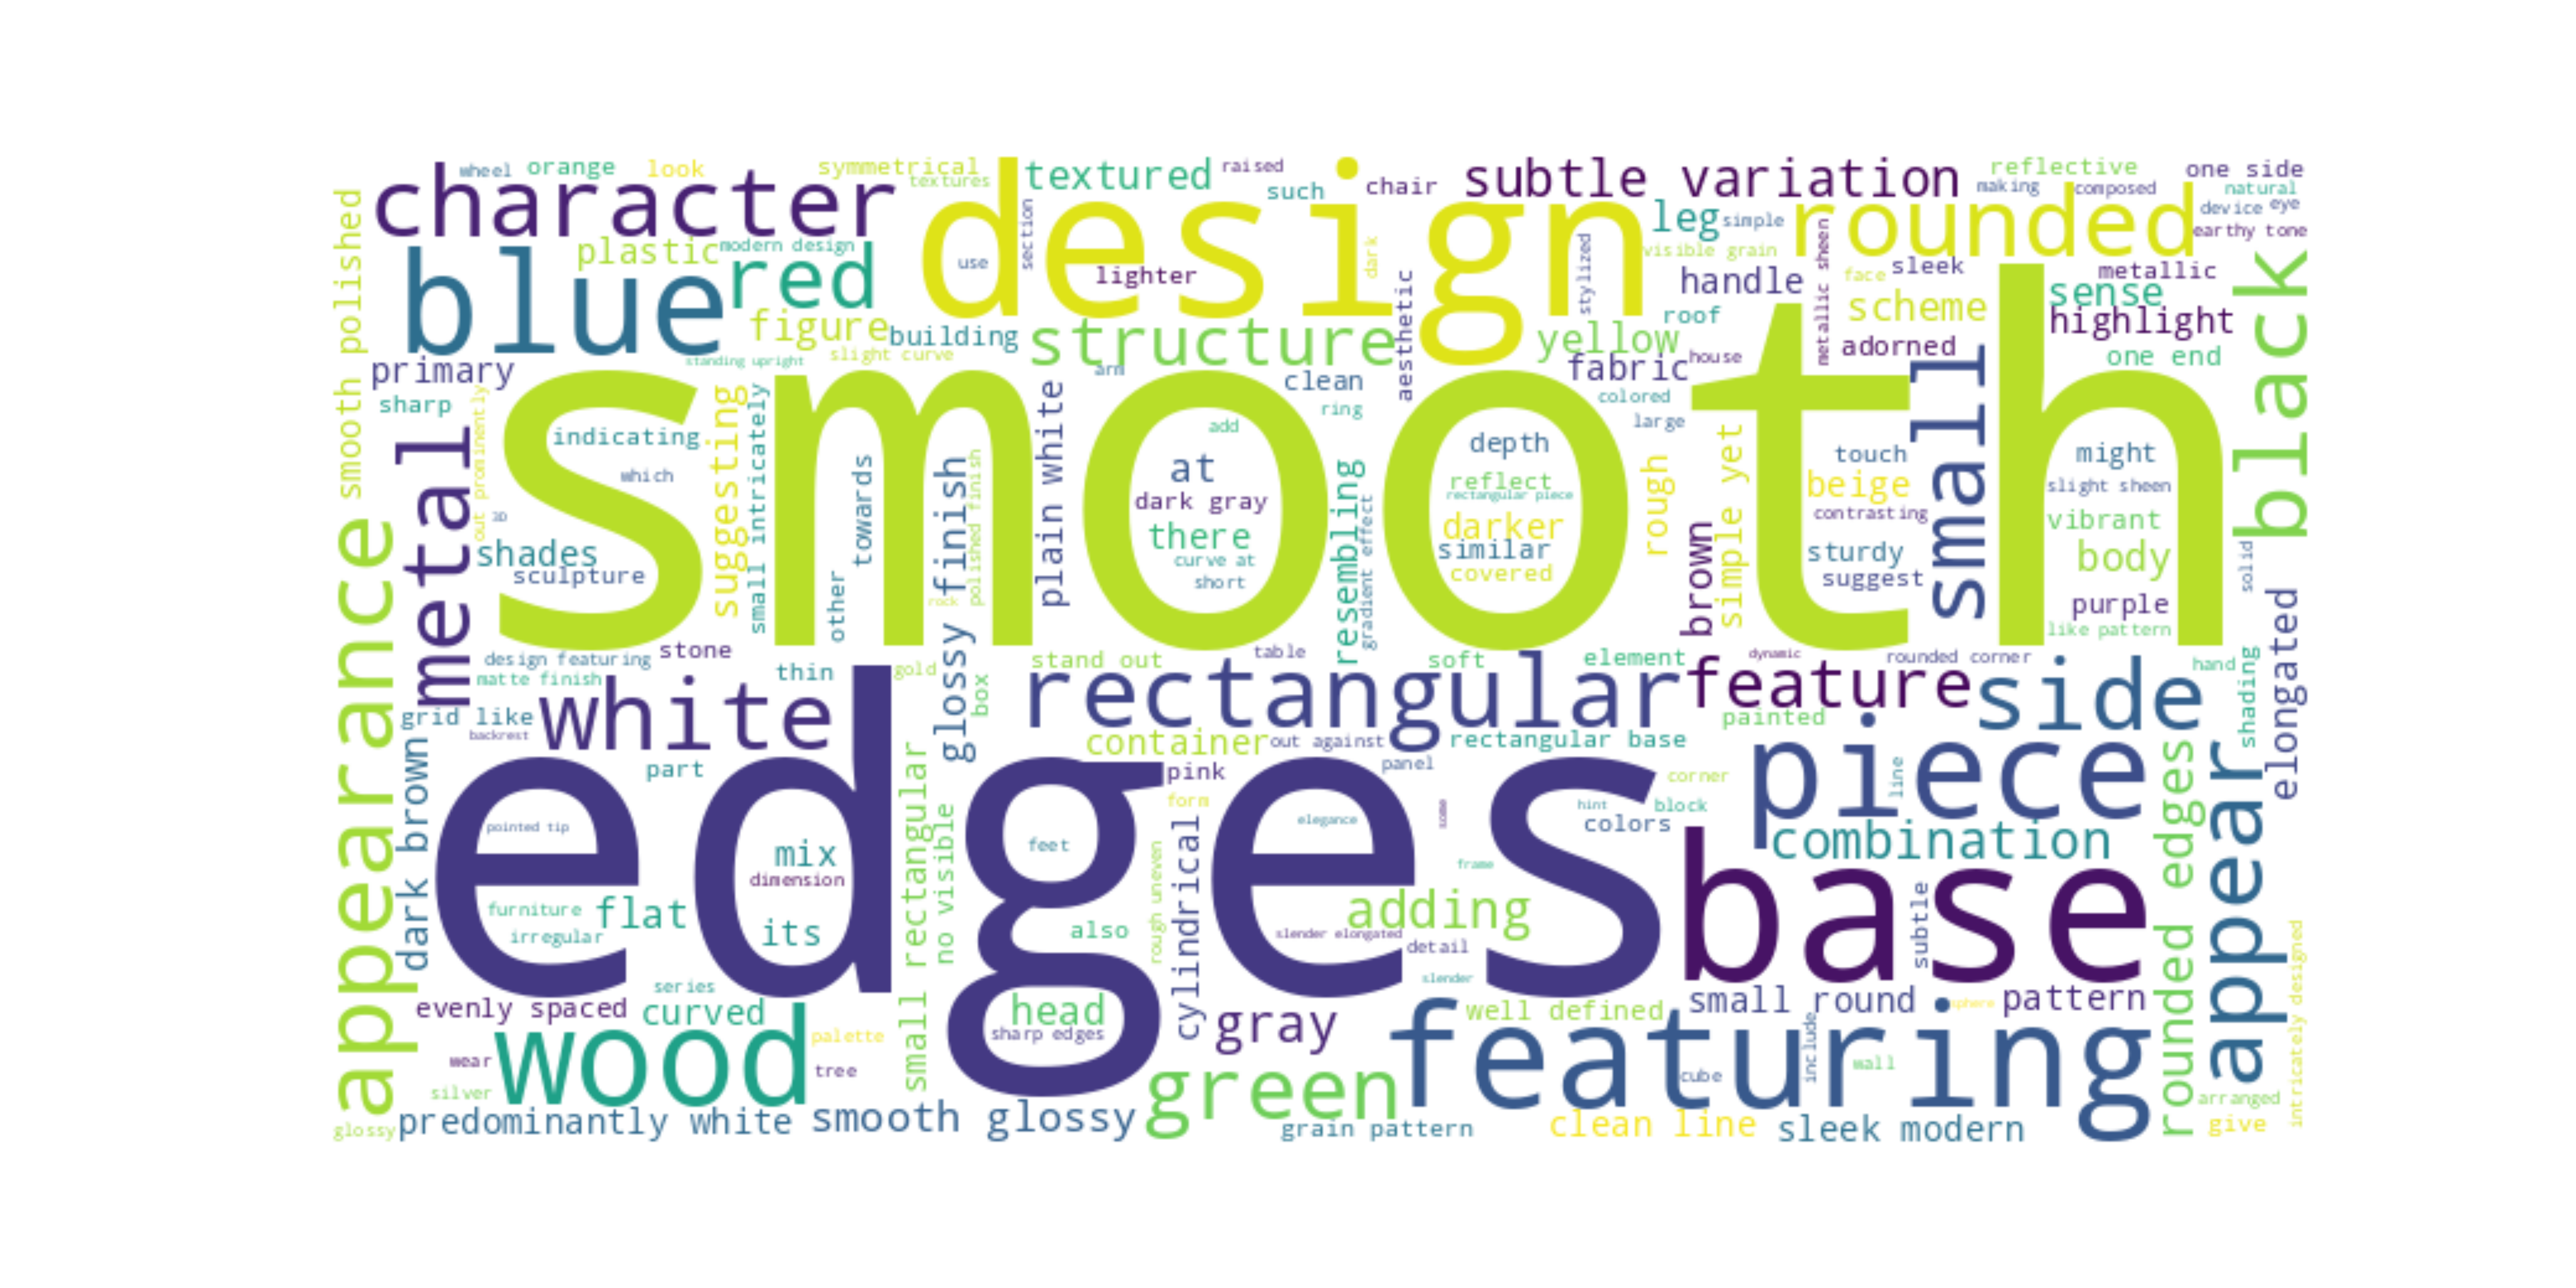
\includegraphics[width=0.8\textwidth]{images/data/objaverse_visualizations/wordcloud_prompts.png}
  \caption{Word cloud of terms from generated prompts.}
  \label{fig:wordcloud-prompts}
\end{figure}

Finally, Table \ref{tab:lda-topics} presents the top 20 topics identified from the textual prompts using Latent Dirichlet Allocation (LDA) \cite{lda}. Each topic is represented by its most characteristic words, providing insight into the semantic clusters present in the dataset's descriptions.

\begin{table}[h]
  \centering
  \caption{Top 20 LDA Topics from Prompts with most characteristic words.}
  \label{tab:lda-topics}
  \begin{tabular}{ll}
    \toprule
    \textbf{Topic} & \textbf{Top Words} \\
    \midrule
    \#1 & evenly, spaced, along, tall, easy, each, crate, rectangular, vertical \\
    \#2 & device, rectangular, edges, rounded, black, small, industrial, panel \\
    \#3 & character, small, body, figure, head, its, eyes, legs, black \\
    \#4 & blue, red, glossy, smooth, vibrant, yellow, white, at, against \\
    \#5 & body, sleek, streamlined, black, design, car, aerodynamic, accents, red \\
    \#6 & metallic, metal, reflective, silver, polished, design, combination, gold, steel \\
    \#7 & base, sculpture, intricately, ceramic, wear, statue, cylindrical, stone, signs \\
    \#8 & box, ring, band, near, rectangular, black, pattern, either, sides \\
    \#9 & green, block, small, tree, leaves, paper, delicate, plant, white \\
    \#10 & well, defined, smooth, sharp, plain, skin, its, white, highlight \\
    \#11 & roof, structure, small, rectangular, wooden, building, house, wood, painted \\
    \#12 & legs, design, frame, chair, wood, backrest, sturdy, dark, seat \\
    \#13 & rectangular, edges, modern, design, smooth, clean, base, white, lines \\
    \#14 & smooth, subtle, brown, wood, rounded, edges, appearance, piece, variations \\
    \#15 & section, part, upper, stick, base, lower, wider, than, more \\
    \#16 & container, fabric, soft, rounded, lid, edges, small, pastel, suitable \\
    \#17 & elongated, end, tapering, towards, rough, one, pointed, at, predominantly \\
    \#18 & which, suggesting, might, indicating, similar, appears, plastic, could, like \\
    \#19 & brown, shades, green, some, small, natural, rough, mix, areas \\
    \#20 & handle, black, sleek, design, cylindrical, finish, modern, smooth, body \\
    \bottomrule
  \end{tabular}
\end{table}

These visualizations and statistics collectively provide a comprehensive overview of the dataset's characteristics, underscoring its suitability for the research presented in this thesis.

\subsection{Dataset Samples}\label{ssec:dataset-samples}
This section presents a selection of samples from the ObjaverseXL dataset. The samples are chosen to showcase the diversity of the dataset and the quality of the rendered views.
